\chapter{從路徑積分到傳播子與頂點}

在介紹粒子及其相互作用之前，值得先釐清這個核心構造。拉格朗日量不只描述經典場方程；透過路徑積分，它也能給出粒子傳播、分裂、結合與散射的振幅。這是從量子場論通往費曼圖最直接的途徑。

\section{粒子與場的最小作用量原理}

費曼路徑積分是最小作用量原理的量子對應。先從一個普通的牛頓力學粒子開始，其拉格朗日量取決於座標與速度：
\begin{equation}
\mathcal{L}=\mathcal{L}(x,\dot{x}),
\end{equation}
一條軌跡所對應的作用量為
\begin{equation}
S[x]=\int \mathcal{L}(x,\dot{x})\,dt.
\end{equation}
從一個時空點到另一個時空點的每一條候選軌跡都有作用量，無論它是否滿足牛頓方程。經典軌跡的特徵是作用量取駐值。按照傳統的``最小作用量''說法，作用量在這條軌跡上取極小值；不過，取駐值才是較一般的表述。駐值條件給出經典微分運動方程。

\begin{figure}[htbp]
\centering
\includegraphics[width=0.72\textwidth]{lecture_10_figure_02.png}
\caption{粒子軌跡的作用量積分。}
\lectureframe{00:02:14}
\end{figure}

同樣的結構也適用於經典場。將所有場統稱為\(\phi\)。局域場拉格朗日密度可以取決於場，以及場的空間與時間導數：
\begin{equation}
\mathcal{L}
=\mathcal{L}\!\left(\phi,\frac{\partial\phi}{\partial x^\mu}\right)
=\mathcal{L}(\phi,\partial_\mu\phi).
\end{equation}
相對論要求\(\mathcal{L}\)在洛倫茲變換下為純量。在此要求下，由場及其導數構成的純量組合，便是拉格朗日量中可能出現的項。

\begin{figure}[htbp]
\centering
\includegraphics[width=0.62\textwidth]{lecture_10_figure_03.png}
\caption{場拉格朗日量對場及其時空導數的依賴。}
\lectureframe{00:04:09}
\end{figure}

對場而言，作用量是在一個時空區域上積分：
\begin{equation}
S[\phi]=\int_{\Omega} d^4x\,\mathcal{L}(\phi,\partial_\mu\phi),
\qquad
d^4x=dt\,dx\,dy\,dz.
\end{equation}
粒子的作用量是沿著一條路徑對時間積分；場的作用量則是在一個時空區域內，對拉格朗日密度積分。

粒子路徑端點固定的對應做法，是指定初始與最終時間切片上的完整場組態。若初始場為\(\phi_{\mathrm{i}}(\mathbf{x})\)，最終場為\(\phi_{\mathrm{f}}(\mathbf{x})\)，那麼插值場便填滿兩者之間的整個時空區域。若邊界資料允許存在經典插值解，則在邊界組態固定時，該解是作用量的駐點。
\editorialnote{兩個時間切片上的任意完整場組態，未必都允許存在經典解。因此，作用量取駐值的敘述僅適用於存在插值解的邊界資料。}

這個幾何結構是粒子路徑在場論中的對應物。\footnote{時空區域示意圖取自約00:04:29的畫面。}
\begin{figure}[htbp]
\centering
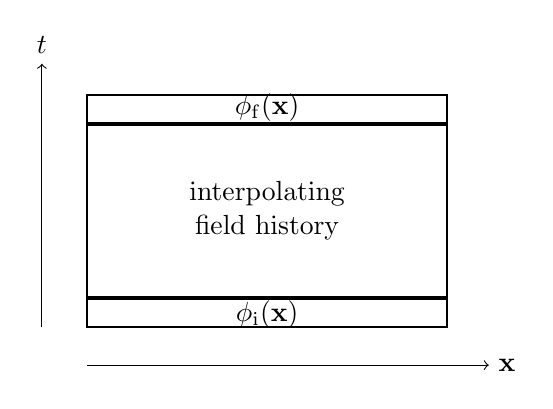
\begin{tikzpicture}[scale=0.88]
\draw[->] (-0.65,0) -- (-0.65,3.8) node[above] {$t$};
\draw[->] (0,-0.55) -- (5.8,-0.55) node[right] {$\mathbf{x}$};
\draw[thick] (0,0) rectangle (5.2,3.35);
\draw[very thick] (0,0.42) -- (5.2,0.42);
\draw[very thick] (0,2.93) -- (5.2,2.93);
\node at (2.6,0.18) {$\phi_{\mathrm{i}}(\mathbf{x})$};
\node at (2.6,3.17) {$\phi_{\mathrm{f}}(\mathbf{x})$};
\node[align=center] at (2.6,1.68) {interpolating\\field history};
\end{tikzpicture}
\caption{界定時空區域的初始與最終場組態。}
\end{figure}

\begin{classroomqa}
\lecturetimestamp{00:07:34}
\audiencequestion{場能回到先前的同一個值嗎？}
\lecturerresponse{可以。場回到先前的值並無障礙，就像粒子的座標可以回到先前的位置一樣。}
\end{classroomqa}

\begin{classroomqa}
\lecturetimestamp{00:07:46}
\audiencequestion{既然邊界資料是場值，為什麼還要談時空事件或軌跡？}
\lecturerresponse{粒子軌跡在此由場的演化歷程取代。場空間中的每個端點，代表選定時間切片上的完整場；而一段歷程則指定兩個切片之間、整個時空區域內每一點的場值。}
\end{classroomqa}

要求插值場的作用量取駐值，會得到偏微分方程。依場與拉格朗日量而定，這些方程包括麥克斯威方程組；對引力作用量而言，則包括愛因斯坦方程。此處不必詳述變分推導；重要的脈絡是
\begin{equation}
\mathcal{L}
\longrightarrow
S[\phi]
\longrightarrow
\text{classical field equations}.
\end{equation}

\section{費曼對粒子路徑的求和}

量子力學不再問哪一條軌跡會發生，而是改問振幅是多少。想像在\((x,t)\)注入一個粒子，閉上眼睛等一會兒，再於\((x',t')\)啟動探測器。振幅
\begin{equation}
\mathcal{A}(x,t;x',t')
\end{equation}
是一個複數，其絕對值的平方就是機率：
\begin{equation}
\begin{aligned}
P(x,t;x',t')
&=\left|\mathcal{A}(x,t;x',t')\right|^2\\
&=\mathcal{A}(x,t;x',t')
\mathcal{A}(x,t;x',t')^*.
\end{aligned}
\end{equation}

費曼規則為每一條候選路徑指定一個作用量，並與之對應一個相位：
\begin{equation}
\exp\!\left(-\frac{i}{\hbar}S[x]\right)
=
\exp\!\left[-\frac{i}{\hbar}\int \mathcal{L}(x,\dot{x})\,dt\right].
\end{equation}

\begin{figure}[htbp]
\centering
\includegraphics[width=0.70\textwidth]{lecture_10_figure_04.png}
\caption{與粒子路徑對應的複數相位。}
\lectureframe{00:11:52}
\end{figure}

因子\(\hbar\)是使指數無量綱所必需的。\footnote{在00:11:52，黑板上的式子自然可讀作\(e^{-i\int\mathcal{L}\,dt}\)；講者則在00:12:02口頭補上因子\(\hbar\)。}躍遷振幅是對所有連接兩端點的可能路徑所對應相位求和：
\begin{equation}
\mathcal{A}(x,t;x',t')
=
\sum_{\substack{\text{paths }x(\tau)\\(x,t)\rightarrow(x',t')}}
\exp\!\left(-\frac{i}{\hbar}S[x]\right).
\end{equation}
此處``可能路徑''不是指牛頓方程的解，而是指求和中包含的任何路徑。在非相對論量子力學中，路徑沿時間向前延伸，不會往回繞行。普朗克常數的量綱是作用量，因此\(S/\hbar\)是無量綱的。

指數形式很自然，因為連續各小步的振幅會相乘。若將一條路徑分成連續的幾段，作用量會相加：
\begin{equation}
S=S_1+S_2+\cdots,
\end{equation}
而相位會相乘：
\begin{equation}
e^{-iS/\hbar}
=e^{-iS_1/\hbar}e^{-iS_2/\hbar}\cdots.
\end{equation}
因子\(i\)不是記帳工具，而是量子力學規則的一部分。

\begin{classroomqa}
\lecturetimestamp{00:13:27}
\audiencequestion{指數形式是否和連續各小步的振幅相乘有關？}
\lecturerresponse{是。連續各步的振幅相乘，而相應的作用量部分則相加。}
\end{classroomqa}

\begin{classroomqa}
\lecturetimestamp{00:13:49}
\audiencequestion{路徑求和本身就是機率嗎？}
\lecturerresponse{不是。路徑求和一般是複數機率振幅；將它乘上複共軛，才得到機率。}
\end{classroomqa}

\section{對場演化歷程求和}

同樣的表述也能延伸至量子場論，不過此處的構造會刻意保持非嚴格的說明方式。從初始場組態\(\phi(\mathbf{x})\)與另行指定的最終場組態\(\phi'(\mathbf{x})\)出發。它們是空間上的完整函數，而不是兩個孤立點上的場值。

可以想像一種理想化裝置，在每個空間點製備場，讓系統演化，之後再測量每個點的場。這種裝置並不實際，但能清楚界定概念上的問題：從初始完整場組態轉變到最終組態的振幅是多少？

每一種可想像的插值場歷程都會有所貢獻。對每一段歷程，計算
\begin{equation}
S[\phi]=\int d^4x\,\mathcal{L}(\phi,\partial_\mu\phi)
\end{equation}
並附上相應的相位。示意地寫成
\begin{equation}
\mathcal{A}\!\left[\phi(\mathbf{x})\rightarrow\phi'(\mathbf{x})\right]
=
\sum_{\substack{\text{field histories}\\
\phi_{\mathrm{i}}=\phi,\;\phi_{\mathrm{f}}=\phi'}}
\exp\!\left(-\frac{i}{\hbar}S[\phi]\right).
\end{equation}
歷程不必是經典場方程的解；它只是在中間時空區域內，對場值所作的一種完整指定。

\begin{classroomqa}
\lecturetimestamp{00:17:39}
\audiencequestion{歷程有無窮多種，而且每個相位的絕對值都是一。它們的總和怎麼會收斂？這些歷程是在取極小值嗎？}
\lecturerresponse{這些歷程是拿來求和，不是取極小值。各項都是分布在單位圓上的相位，因此可以彼此抵消。這和相加無窮多個且遠離零的正項不同。振盪積分可以收斂；傅立葉表示中的狄拉克{\proseunicodefont δ}函數就是熟悉的例子。如果相位均勻分布在圓周上，它們的向量總和會是零。大多數歷程都會強烈抵消。靠近作用量駐值軌跡的歷程抵消得最少，因為那裡的相位變化最慢；經典極限便由此浮現。}
\end{classroomqa}

\editorialnote{實時間路徑積分通常需要指定收斂處方。此處以單位圓說明的是振盪抵消的論證，並非收斂性的一般證明。}

可以把這種抵消想像成複平面上的向量和。\footnote{單位圓的示意取自00:18:32--00:20:21的黑板講解。}
\begin{figure}[htbp]
\centering
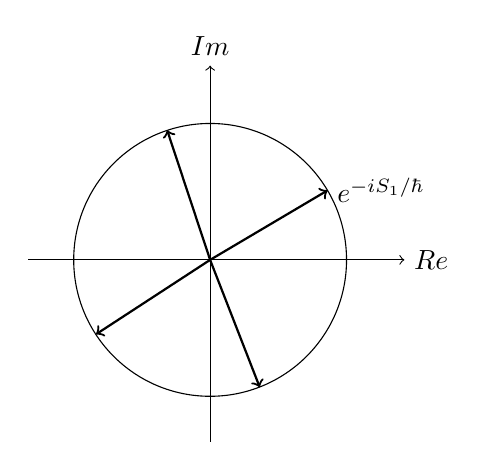
\begin{tikzpicture}[scale=1.05]
\draw[->] (-2.2,0) -- (2.35,0) node[right] {$\operatorname{Re}$};
\draw[->] (0,-2.2) -- (0,2.35) node[above] {$\operatorname{Im}$};
\draw (0,0) circle (1.65);
\draw[thick,->] (0,0) -- (1.42,0.84);
\draw[thick,->] (0,0) -- (-1.38,-0.90);
\draw[thick,->] (0,0) -- (-0.52,1.57);
\draw[thick,->] (0,0) -- (0.60,-1.54);
\node[right] at (1.42,0.84) {$e^{-iS_1/\hbar}$};
\end{tikzpicture}
\caption{當單位長度的相位方向不同時，它們可以彼此抵消。}
\end{figure}

確實如此，
\begin{equation}
e^{-iS/\hbar}
=
\cos\!\left(\frac{S}{\hbar}\right)
-i\sin\!\left(\frac{S}{\hbar}\right).
\end{equation}
每個貢獻都是一個單位向量。方向不同的貢獻既會相加，也會相消。在\(S\)的駐點附近，相鄰歷程的相位幾乎相同，因此各自的貢獻更容易相互增強。遠離作用量駐值處，相位變化快速，破壞性干涉便占上風。

這種路徑積分結構是幾乎所有現代量子場論的基礎。接下來會直接陳述實際計算的下一步，不作推導。這是一種過度簡化的計算入門方式，但能看出同一個對象如何用兩種語言描述。

計算一個物理過程，就是計算從初態到末態的躍遷機率。一種描述方式指定初始場組態與最終場組態；另一種則指定入射與出射粒子，也就是一種或多種場的量子。兩個問題看似不同，計算時卻都使用同一個場論路徑積分。

\section{離散時空形式}

要讓場演化歷程的求和有具體意義，可以將時空切分成小格，並為每一格指定一個場值。縮小格子尺寸便能趨近連續極限，不過目前格子仍維持有限大小。如此一來，對函數所作的形式求和，就轉成對格點上各種數值指定方式求和。

先前有一種啟發式作法：對每一格取一個類似\(1+\mathcal{L}_i\)的因子，將因子相乘，再辨認出描述粒子傳播與碰撞的項。這個構造很重要，值得再次說明，但其中的因子必須修正。小量不是拉格朗日量本身，而是格子內所包含的作用量。

若一格的時空體積為
\begin{equation}
a^4=\Delta t\,\Delta x\,\Delta y\,\Delta z,
\end{equation}
則該格的作用量為
\begin{equation}
A_i=\mathcal{L}_i a^4.
\end{equation}
由於格子很小，\(A_i\)也很小。暫時略去\(\hbar\)後，修正過的基本因子是
\begin{equation}
1-iA_i,
\end{equation}
而不是\(1+\mathcal{L}_i\)。

對任意小的\(\epsilon\)，
\begin{equation}
1+\epsilon\simeq e^\epsilon,
\end{equation}
因為
\begin{equation}
e^\epsilon
=1+\epsilon+\frac{\epsilon^2}{2!}
+\frac{\epsilon^3}{3!}+\cdots.
\end{equation}
因此，在這些暫定的單位下，只要格子夠小，\(1-iA_i\)便近似於\(e^{-iA_i}\)。從一開始就使用精確的指數因子會更簡潔。

\begin{classroomqa}
\lecturetimestamp{00:27:57}
\audiencequestion{指數中需要有\(\hbar\)因子嗎？}
\lecturerresponse{需要。無量綱的格子因子在一階近似下是\(1-iA_i/\hbar\)，精確的指數形式則是\(\exp(-iA_i/\hbar)\)。之後可以採用\(\hbar=1\)的單位。}
\end{classroomqa}

將\(\hbar\)放回後，修正過的中間因子及其指數形式為
\begin{equation}
1-\frac{i}{\hbar}A_i
\simeq
\exp\!\left(-\frac{i}{\hbar}A_i\right).
\end{equation}

對一段固定的歷程，將時空積分換成各格作用量的總和：
\begin{equation}
S[\phi]
=\int d^4x\,\mathcal{L}
\;\longrightarrow\;
\sum_i A_i.
\end{equation}
該歷程所對應的相位變為
\begin{equation}
\exp\!\left(-\frac{i}{\hbar}\sum_i A_i\right).
\end{equation}
總和的指數等於各指數的乘積：
\begin{equation}
\exp\!\left(-\frac{i}{\hbar}\sum_i A_i\right)
=
\prod_i\exp\!\left(-\frac{i}{\hbar}A_i\right).
\end{equation}
運算順序很重要。先選定一段完整歷程，將它在各格上的權重相乘；之後才對不同歷程求和。

格點結構也讓邊界資料一目了然。\footnote{棋盤格及固定的首末列示意取自約00:23:54和00:30:49的畫面。}
\begin{figure}[htbp]
\centering
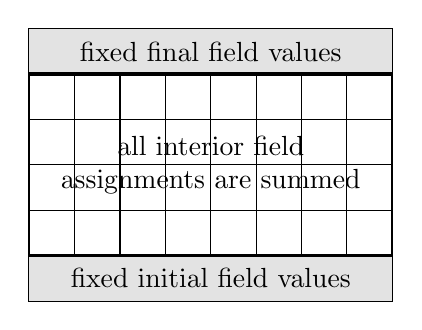
\begin{tikzpicture}[scale=0.72]
\draw[step=0.8,thin] (0,0) grid (6.4,4.8);
\draw[thick] (0,0) rectangle (6.4,4.8);
\fill[gray!22] (0,0) rectangle (6.4,0.8);
\fill[gray!22] (0,4.0) rectangle (6.4,4.8);
\draw[very thick] (0,0.8) -- (6.4,0.8);
\draw[very thick] (0,4.0) -- (6.4,4.0);
\node at (3.2,0.4) {fixed initial field values};
\node at (3.2,4.4) {fixed final field values};
\node[align=center] at (3.2,2.4) {all interior field\\assignments are summed};
\end{tikzpicture}
\caption{初始與最終格點列固定的離散場歷程。}
\end{figure}

第一列指定初始場組態，最後一列指定最終場組態。每個內部格子都可以取離散化所包含的任一場值。因此，躍遷振幅的示意形式為
\begin{equation}
\mathcal{A}\!\left[\phi_{\mathrm{i}}\rightarrow\phi_{\mathrm{f}}\right]
=
\sum_{\{\phi\}_{\mathrm{interior}}}
\prod_i\exp\!\left(-\frac{i}{\hbar}A_i[\phi]\right),
\end{equation}
其中首末兩列保持固定。換句話說，對每一種內部格點賦值，計算總作用量的指數，再將該貢獻加上其他所有賦值所對應的貢獻。

\section{從場組態到粒子組態}

同一個躍遷振幅可以用場來描述，也可以用粒子來描述。除了固定第一與最後一個時間切片上的場，也可以指定入射與出射的場量子集合，並求出連接兩者的振幅。所計算的對象相同，改變的只有邊界描述。

量子場包含產生算符與湮滅算符。因此，場的乘積作用於粒子態時，可以產生、湮滅或移動量子。正是這種算符解讀，讓格點路徑積分轉化成一套粒子規則。

\begin{classroomqa}
\lecturetimestamp{00:34:11}
\audiencequestion{場量子是否必然能辨認為粒子？}
\lecturerresponse{不一定能以傳統方式辨認為可分別觀測的粒子。例如，夸克是夸克場的量子，但夸克禁閉使孤立夸克無法脫離其他夸克而被單獨探測。更一般地，理論中所列的場與以傳統方式可觀測的粒子種類，不必一一對應。有些場論並不容許這種簡單的對應關係。如果``粒子''一詞廣義地指攜帶能量及其他量子數、不可再分的量子，那麼兩者的區別有一部分可能只是術語上的差異。}
\end{classroomqa}

\editorialnote{來源在00:35:45--00:36:08處提到弱耦合，但語法有歧義，此處無法判定其意。可以確定的是，場的標記與傳統上可觀測的粒子種類不必一一對應。}

格點求和仍然遍歷各種場值，並未限於類似光滑經典解的組態。

\begin{classroomqa}
\lecturetimestamp{00:36:44}
\audiencequestion{場的歷程必須連續，或至少近似連續嗎？}
\lecturerresponse{不必。在離散格點上，相鄰格子各自帶有場值，而所有賦值都納入求和，並不要求歷程近似連續。量子場會劇烈漲落；典型歷程並非光滑的經典場。}
\end{classroomqa}

獨立指定的變數是格點或格子上的場值。導數則由相鄰場值之差計算而得。

\begin{classroomqa}
\lecturetimestamp{00:37:56}
\audiencequestion{場及其導數是分別獨立指定的嗎？}
\lecturerresponse{不是。指定的是格點上的場值，之後再由相鄰場值之差重建導數。有限差分可以有不同的定義方式，但導數不是額外的獨立變數。}
\end{classroomqa}

因此，若格點間距為\(a\)，可以示意地寫成
\begin{equation}
\partial_\mu\phi(x)
\longrightarrow
\frac{\phi(x+a\hat\mu)-\phi(x)}{a}.
\end{equation}
場值軸本身也可以切分成小區間，讓每個格點上有可數多種可能的場值。

\begin{classroomqa}
\lecturetimestamp{00:38:53}
\audiencequestion{如果場不只一種，會有什麼變化？}
\lecturerresponse{每個格點上都要為每一種場指定一個值，而求和則遍歷所有這類賦值。}
\end{classroomqa}

複值場不可與複變數的解析函數混為一談。解析性是極為嚴格的光滑條件。場路徑積分中的歷程不必滿足這個條件，一般而言甚至不近似光滑。

\begin{classroomqa}
\lecturetimestamp{00:39:07}
\audiencequestion{若場的值是複數，是否也必須滿足解析函數所具備的光滑條件？}
\lecturerresponse{不必。複值不代表解析。解析函數理論研究的是極其光滑、受到嚴格限制的一類函數。此處納入求和的歷程不必是位置的解析函數；典型歷程高度不規則，在連續極限下甚至可視為高度不連續。}
\end{classroomqa}

這樣的計算看來十分艱鉅。即使時空和場值都已離散化，仍可能有極其龐大的賦值數量需要取樣。

\begin{classroomqa}
\lecturetimestamp{00:40:04}
\audiencequestion{電腦如何知道要取樣多少種格點賦值，或何時算是收斂？}
\lecturerresponse{這屬於格點規範理論，或者更廣泛地說，屬於格點量子場論。如今它已是一門成熟的計算領域。我在格點規範理論發展初期參與建立規則，並未參與後來的電腦技術。建立規則花了大約三週；發展計算這些問題所需的技術，則花了大約三十年。許多實務經驗來自統計力學；在統計力學中，配分函數也是藉由對格點組態求和得到的---例如，對晶體中某格點是否被佔據求和。要判斷取樣的組態是否足夠，是一項技術問題。專家知道---或認為自己知道---如何判斷計算是否受到妥善控制，而所得計算結果與實驗相符。}
\end{classroomqa}

格點規範理論的概念規則很快就建立起來；使用這些規則進行計算所需的技術，則花了長得多的時間。棋盤格不只是類比，也是實用計算方法的起點。

\section{二次項與粒子傳播}

現在回到場的算符詮釋。對兩個相鄰格點\(x\)與\(x'\)而言，乘積
\begin{equation}
\phi(x)\phi(x')
\end{equation}
在適當的單粒子矩陣元中，可以表示在一個格點湮滅粒子、並在另一個格點產生粒子。因此，在該粒子扇區中，可以將它想成一次跨越單一連結的躍遷。這只是對算符乘積的一種詮釋，並非唯一的解讀。

導數項會形成這類連結。嚴格來說，它們並非與單一格子相聯，而是與一對相鄰格點相聯。例如，時間導數會變成
\begin{equation}
\partial_t\phi(t,\mathbf{x})
\longrightarrow
\frac{\phi(t+a,\mathbf{x})-\phi(t,\mathbf{x})}{a},
\end{equation}
空間導數也以同樣方式沿著空間方向的連結處理。

\begin{classroomqa}
\lecturetimestamp{00:44:39}
\audiencequestion{這裡討論的拉格朗日量含有二階導數嗎？}
\lecturerresponse{此處所談的標準理論以一階導數表示，因此其格點版本使用相鄰格點之間的一階差分。}
\end{classroomqa}

將一階差分平方，會同時產生同一格點上的項與相鄰格點間的交叉項：
\begin{align}
\frac{1}{2}\bigl[\phi(x)-\phi(x')\bigr]^2
&=
\frac{1}{2}\phi(x)^2
+\frac{1}{2}\phi(x')^2
-\phi(x)\phi(x').
\end{align}
交叉項可以表示粒子從一個格點移動到另一個格點。兩個平方項則各自只涉及同一格點。二次導數項是動能項；接下來會先利用其中涉及相鄰格點的交叉項來建構傳播。

為了單獨看出組合結構，將相鄰格點的乘積收集為
\begin{equation}
K=\sum_{\langle x,x'\rangle}\phi(x)\phi(x').
\end{equation}
路徑積分權重中相應的因子可示意地寫成
\begin{equation}
e^{-iK}.
\end{equation}
\editorialnote{這個示意格點因子省略了格點間距的冪次\(\hbar\)、度規符號、歸一化常數與各連結的係數。}
其展開為
\begin{equation}
e^{-iK}
=1-iK-\frac{1}{2!}K^2+\frac{i}{3!}K^3+\cdots,
\end{equation}
或者將相鄰格點的求和明確寫出：
\begin{align}
e^{-iK}
={}&1
-i\sum_{\langle x,x'\rangle}\phi(x)\phi(x')
\nonumber\\
&-\frac{1}{2!}
\sum_{\langle x,x'\rangle}
\sum_{\langle y,y'\rangle}
\phi(x)\phi(x')\phi(y)\phi(y')
+\cdots .
\end{align}
每個因子都會獨立選取一對相鄰格點。

粒子圖遵守端點不可懸空的規則。只有在邊界條件明確於初始切片插入粒子，或於最終切片移除粒子時，才允許端點露出。內部單獨一條連結的兩端未配對，不能構成對指定躍遷的完整貢獻。內部連結的端點必須接合。

先考慮只有兩個時間層的格點。若初態在\(x\)插入粒子，而末態在相鄰位置\(x'\)移除粒子，一階項便能連接這兩個邊界插入：
\begin{equation}
x\longrightarrow x',
\qquad
\mathcal{A}_{\text{one link}}\sim -i.
\end{equation}
係數\(-i\)只是這個示意展開中的係數；格點因子與歸一化因子雖然省略，仍隱含其中。

\begin{classroomqa}
\lecturetimestamp{00:52:16}
\audiencequestion{一階的單連結項是否只有在相關的初態與末態格點相鄰時才有貢獻？}
\lecturerresponse{是。該項選取一對相鄰格點，所以只有當兩個邊界格點彼此相鄰時，才能連接它們。更遠距離的傳播來自高階乘積。}
\end{classroomqa}

在二階項中，兩個因子各自對相鄰格點對求和，彼此獨立：
\begin{equation}
K^2
=
\sum_{\langle x,x'\rangle}
\sum_{\langle y,y'\rangle}
\phi(x)\phi(x')\phi(y)\phi(y').
\end{equation}

\begin{classroomqa}
\lecturetimestamp{00:52:40}
\audiencequestion{第二個相鄰格點對是否必須接在第一個因子選取的格點對旁邊？}
\lecturerresponse{不必。每個因子都獨立選取一對相鄰格點。兩對格點可以共用一個格點、完全分開，甚至可以是同一對格點。求和涵蓋所有可能性。}
\end{classroomqa}

對一個粒子跨越三個時間層的傳播而言，有用的二階選取會共用一個中間格點：
\begin{equation}
\bigl[\phi(x_0)\phi(x_1)\bigr]
\bigl[\phi(x_1)\phi(x_2)\bigr],
\qquad
x_0\longrightarrow x_1\longrightarrow x_2.
\end{equation}
第一條連結的末端接上第二條連結的起點。只有\(x_0\)處的初始端點與\(x_2\)處的最終端點仍然露出，因此這一項會對所需的單粒子躍遷有所貢獻。在指數的示意展開中，其係數為
\begin{equation}
-\frac{1}{2!}.
\end{equation}

選取結果也可能形成彼此分開的躍遷。\footnote{連結圖取自00:49:18--00:55:12的講解序列。}
\begin{figure}[htbp]
\centering
\resizebox{\linewidth}{!}{%
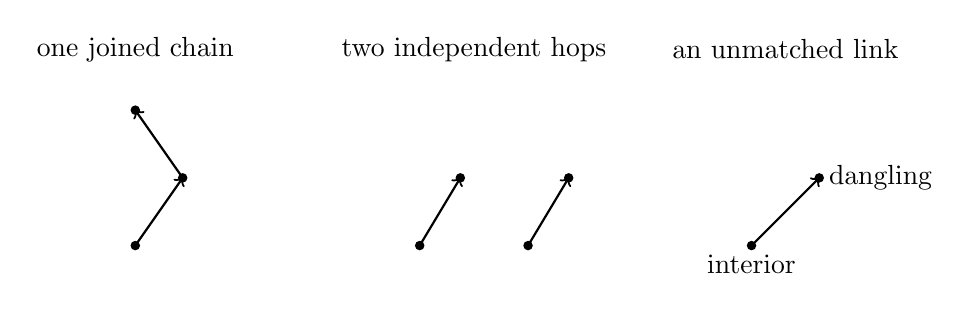
\begin{tikzpicture}[scale=0.86]
\node at (0,2.9) {one joined chain};
\fill (0,0) circle (2pt);
\fill (0.7,1.0) circle (2pt);
\fill (0,2.0) circle (2pt);
\draw[thick,->] (0,0) -- (0.7,1.0);
\draw[thick,->] (0.7,1.0) -- (0,2.0);

\begin{scope}[xshift=4.2cm]
\node at (0.8,2.9) {two independent hops};
\fill (0,0) circle (2pt);
\fill (0.6,1.0) circle (2pt);
\fill (1.6,0) circle (2pt);
\fill (2.2,1.0) circle (2pt);
\draw[thick,->] (0,0) -- (0.6,1.0);
\draw[thick,->] (1.6,0) -- (2.2,1.0);
\end{scope}

\begin{scope}[xshift=9.1cm]
\node at (0.5,2.9) {an unmatched link};
\fill (0,0) circle (2pt);
\fill (1.0,1.0) circle (2pt);
\draw[thick,->] (0,0) -- (1.0,1.0);
\node[below] at (0,0) {interior};
\node[right] at (1.0,1.0) {dangling};
\end{scope}
\end{tikzpicture}%
}
\caption{接合、彼此獨立，以及端點未配對的相鄰連結選取。}
\end{figure}

在這個階數上，已經可能有不只一條路徑。若位移一個時間方向的格點步長與一個空間方向的格點步長，以下兩種順序
\begin{align}
x
&\longrightarrow x+\hat t
\longrightarrow x+\hat t+\hat s,\\
x
&\longrightarrow x+\hat s
\longrightarrow x+\hat s+\hat t
\end{align}
都會抵達同一個端點。

\begin{classroomqa}
\lecturetimestamp{00:55:53}
\audiencequestion{還有另一條兩步路徑能到達同一個對角端點嗎？}
\lecturerresponse{有。可以先走時間方向的一步，再走空間方向的一步；也可以反過來。兩條路徑都會對同一個躍遷振幅有所貢獻。}
\end{classroomqa}

路徑不必止於兩條連結。三階項會提供由三條相鄰連結構成的路徑鏈。路徑可以直接前進、繞道，或先離開再折返，最後抵達終點。更高階項則包含更長的繞道與反覆折返。因此，展開至任意階，便會為每一條由局部連結組成的路徑帶來一項貢獻。兩點之間的振幅是所有這些貢獻的總和，其係數包含\(i\)的適當次方與階乘：
\begin{equation}
\begin{gathered}
\mathcal{A}(x_{\mathrm{in}}\to x_{\mathrm{out}})
=
\sum_{\text{joined lattice routes }r}c_r,
\\
c_r\ \hbox{read from the exponential expansion}.
\end{gathered}
\end{equation}
這些係數一般是複數，因此所得振幅也是複數。

相對論性傳播還多出一種可能性：路徑可以沿時間方向先向上再向下，也可以反覆經過同一條連結。

\begin{classroomqa}
\lecturetimestamp{00:58:47}
\audiencequestion{一條路徑能不能反覆穿過同樣兩個格點？}
\lecturerresponse{可以。路徑可以反覆穿越；在相對論性展開中，也可以沿時間反方向延伸。}
\end{classroomqa}

時間向後延伸的線段有兩種等價的圖像解讀。可以把它視為一條沿時間反向延伸的粒子線。也可以只沿時間正向追蹤：產生一對粒子--反粒子，其中粒子繼續向前傳播，而反粒子隨後與原來的粒子相遇並湮滅。同一條連通線能表達這兩種描述。\footnote{這兩種解讀依循00處的圖示與說明：59：00--00：59：51。}

\begin{figure}[htbp]
\centering
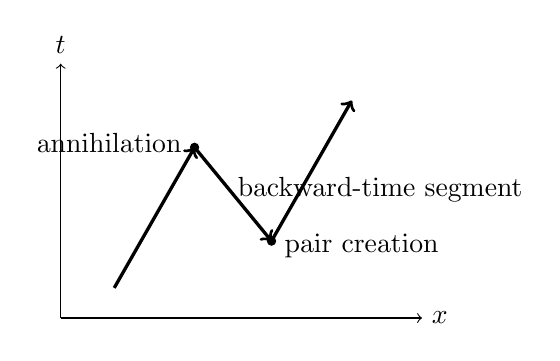
\begin{tikzpicture}[scale=0.85]
\draw[->] (0,0) -- (0,3.8) node[above] {$t$};
\draw[->] (0,0) -- (5.4,0) node[right] {$x$};
\draw[very thick,->] (0.8,0.45) -- (2.0,2.55);
\draw[very thick,->] (2.0,2.55) -- (3.15,1.15);
\draw[very thick,->] (3.15,1.15) -- (4.35,3.25);
\fill (2.0,2.55) circle (2pt);
\fill (3.15,1.15) circle (2pt);
\node[left] at (1.95,2.62) {annihilation};
\node[right] at (3.20,1.08) {pair creation};
\node[right] at (2.50,1.92) {backward-time segment};
\end{tikzpicture}
\caption{時間向後延伸的線段，若按時間正向解讀，代表粒子對的產生與湮滅。}
\end{figure}

高階項中出現的階乘控制著指數冪級數，但這不等於控制對所有場組態的完整求和。

\begin{classroomqa}
\lecturetimestamp{01:00:00}
\audiencequestion{\(1/n!\)這些因子能保證收斂嗎？}
\lecturerresponse{它們能保證自變數固定時指數級數收斂，但本身不能保證對所有場組態分別求和時也會收斂。這是兩個不同的問題。在場值經過有限離散化的有限點陣上，組態數目有限；但連續極限與無限體積極限仍需要進一步控制。}
\end{classroomqa}

\section{一個連線乘積，多種粒子解讀}

二階乘積所包含的，不只有單粒子傳播。當其中兩個相鄰對共用一個端點時，它可以讓一個粒子沿兩條連線組成的鏈移動：
\begin{equation}
\bigl[\phi(x_0)\phi(x_1)\bigr]
\bigl[\phi(x_1)\phi(x_2)\bigr].
\end{equation}
當選取的兩對彼此分開時，同一個二階項也可以讓兩個粒子各自移動一條連線。\footnote{單粒子傳播與兩次彼此獨立的單連線跳躍之比較，是根據01處的板書討論重構而成：00：46--01：02：34。}
\begin{equation}
\bigl[\phi(x_0)\phi(x_1)\bigr]
\bigl[\phi(y_0)\phi(y_1)\bigr],
\qquad x_0\neq y_0.
\end{equation}
第一個因子傳播一個粒子，第二個因子則傳播另一個粒子。因此，點陣上的二次展開包含所有多粒子扇區中的傳播振幅。同一個代數階既可以描述一條較長的連通路徑，也可以描述數條較短的非連通路徑。

這裡包含許多資訊，但還沒有真正的相互作用頂點。只有二次傳播項時，連通的粒子線不會分裂成數目不同的線。改變粒子數的過程需要額外的相互作用，儘管局域算符乘積可能有幾種產生與湮滅的解讀方式。

\begin{classroomqa}
\lecturetimestamp{01:03:30}
\audiencequestion{電子和正電子能不能湮滅，最後不留下任何粒子？}
\lecturerresponse{若入射能量非零，而末態中沒有任何攜帶能量的粒子，這樣的貢獻便違反能量守恆。對頂點可能出現的時空位置求和時，各位置的振幅會彼此抵消。若有另一個場帶走能量，電子--正電子就可以湮滅---例如產生電磁量子。}
\end{classroomqa}

\editorialnote{簡略的交換推導直接從二次跳躍轉到電子--正電子湮滅。應明確區分的是：二次項提供自由傳播；物理上的湮滅則需要與另一個場發生相互作用。若沒有能量輸出的振幅會因能量守恆而抵消。}

因此，導數項雖然涵蓋許多內容，卻不是全部。拉格朗日量中的其他項，則由實驗觀測到的場之性質與相互作用決定。

\section{質量項}

對於標量場，此處討論的導數結構具有如下示意性的洛倫茲符號形式：
\begin{equation}
\mathcal{L}_{\mathrm{kin}}
\sim
\frac{1}{2}\left[
(\partial_t\phi)^2
-(\partial_x\phi)^2
-(\partial_y\phi)^2
-(\partial_z\phi)^2
\right].
\end{equation}
這個式子確立了本段討論所需的時間項減去空間項之結構；整體符號與歸一化慣例則未明示。

拉格朗日量也可以包含未微分場的各次方。二次項的一個例子如下：
\begin{equation}
\text{mass term}\ \propto\ \frac{1}{2}m^2\phi^2,
\end{equation}
其中\(m^2\)表示質量係數。\editorialnote{這段原文未指定完整標量拉格朗日量的整體符號慣例。}在示意性的粒子解讀中，此項會湮滅一個粒子，再於同一個點陣位置將它重新產生。它不會使粒子位移，而是在路徑中插入一個同一位置的因子：
\begin{equation}
\text{particle at }x
\longrightarrow
\boxed{m^2\phi(x)^2}
\longrightarrow
\text{particle still at }x.
\end{equation}
每次這種插入作用時，路徑便會多出一個正比於\(m^2\)的因子。

若只保留導數項，這個示意性展開所描述的傳播就是無質量理論。對有質量的場而言，路徑可以在各跳躍項之間包含任意多次同一位置的質量插入。質量項會改變各條路徑的相對權重，使所得傳播子帶有粒子的質量。

\section{三次項與分裂--重新合併的歷程}

質量項會改變路徑的權重，但不會移動粒子。次數高於二次的項則會帶來更有趣的行為。考慮一個三次相互作用：
\begin{equation}
\mathcal{L}_{\mathrm{int}}=g_3\phi^3.
\end{equation}
在一個格點上，三個場因子有四種粒子解讀方式：
\begin{equation}
1\longrightarrow 2,
\qquad
2\longrightarrow 1,
\qquad
0\longrightarrow 3,
\qquad
3\longrightarrow 0.
\end{equation}
因此，三次因子可以湮滅一個粒子並產生兩個、湮滅兩個並產生一個、產生三個，或湮滅三個。

相鄰成對的二次因子仍然提供傳播。一連串這類因子可以把一個粒子帶到某個格點；該處的三次因子可以吸收它並放出兩個粒子，接著其他二次因子再把這兩個粒子傳播出去。這會對一個入射粒子、兩個出射粒子的振幅有所貢獻。\footnote{點陣幾何依據01處的圖示重構而成：08：48--01：09：42。}

\begin{figure}[htbp]
\centering
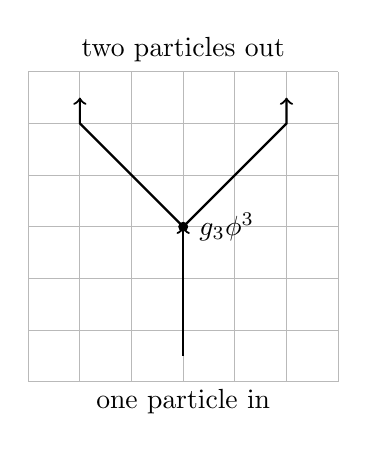
\begin{tikzpicture}[scale=0.82]
\draw[step=0.8,gray!55,thin] (0,0) grid (4.8,4.8);
\draw[thick,->] (2.4,0.4) -- (2.4,1.2) -- (2.4,2.0) -- (2.4,2.4);
\fill (2.4,2.4) circle (2.2pt);
\draw[thick,->] (2.4,2.4) -- (1.6,3.2) -- (0.8,4.0) -- (0.8,4.4);
\draw[thick,->] (2.4,2.4) -- (3.2,3.2) -- (4.0,4.0) -- (4.0,4.4);
\node[right] at (2.5,2.4) {$g_3\phi^3$};
\node at (2.4,-0.3) {one particle in};
\node at (2.4,5.15) {two particles out};
\end{tikzpicture}
\caption{二次因子將粒子傳播至三次分裂頂點，並從該頂點傳播出去。}
\end{figure}

即使初態和末態都各有一個粒子，振幅也不再只是單一、不間斷路徑的總和。一種貢獻來自一連串二次跳躍所形成的直接傳播；另一種則包含兩個三次因子：粒子先分裂成兩個，之後這兩個粒子再度合併。因此，中間態的粒子數可以多於外態。\footnote{這兩種情形依據01處的圖示重構而成：09：44--01：11：36。}

\begin{figure}[htbp]
\centering
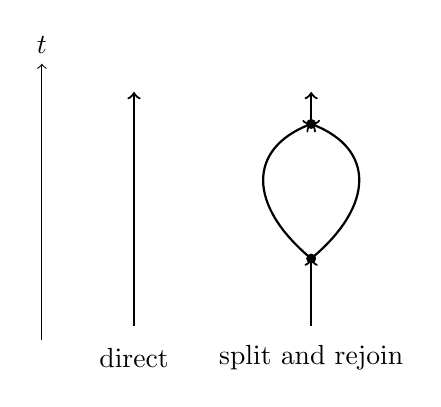
\begin{tikzpicture}[scale=0.9]
\draw[->] (-0.7,0) -- (-0.7,3.9) node[above] {$t$};
\draw[thick,->] (0.6,0.2) -- (0.6,3.5);
\node at (0.6,-0.25) {direct};
\draw[thick,->] (3.1,0.2) -- (3.1,1.15);
\fill (3.1,1.15) circle (2pt);
\draw[thick,->] (3.1,1.15) .. controls (2.2,1.9) and (2.2,2.7) .. (3.1,3.05);
\draw[thick,->] (3.1,1.15) .. controls (4.0,1.9) and (4.0,2.7) .. (3.1,3.05);
\fill (3.1,3.05) circle (2pt);
\draw[thick,->] (3.1,3.05) -- (3.1,3.5);
\node at (3.1,-0.25) {split and rejoin};
\end{tikzpicture}
\caption{對同一個單粒子振幅的直接傳播與分裂--重新合併貢獻。}
\end{figure}

在電動力學中，相應的例子是電子發射一個光子，之後再將它吸收。這段先發射再吸收的歷程，是電子從一點傳播到另一點之振幅的一部分。高階項則包含多次發射與吸收。光子可以轉化成電子--正電子對，而這個中間態中的電子與正電子本身也可以交換光子。初態和末態的粒子內容簡單，並不表示中間態的粒子內容也必然簡單。\footnote{以下重構中的例子出現在01：11：22--01：12：34。}

\begin{figure}[htbp]
\centering
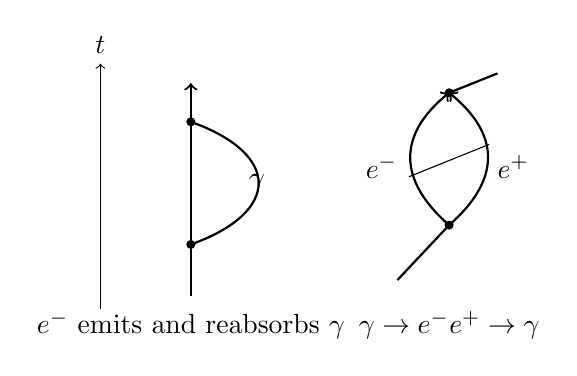
\begin{tikzpicture}[scale=0.82]
\draw[->] (-0.6,0) -- (-0.6,3.8) node[above] {$t$};
\draw[thick,->] (0.8,0.2) -- (0.8,3.5);
\fill (0.8,1.0) circle (2pt);
\fill (0.8,2.9) circle (2pt);
\draw[thick] (0.8,1.0) .. controls (2.2,1.5) and (2.2,2.4) .. (0.8,2.9);
\node[right] at (1.55,1.95) {$\gamma$};
\node at (0.8,-0.25) {$e^-$ emits and reabsorbs $\gamma$};
\draw[thick] (4.0,0.45) -- (4.8,1.3);
\fill (4.8,1.3) circle (2pt);
\draw[thick,->] (4.8,1.3) .. controls (4.0,2.0) and (4.0,2.7) .. (4.8,3.35);
\draw[thick,->] (4.8,1.3) .. controls (5.6,2.0) and (5.6,2.7) .. (4.8,3.35);
\fill (4.8,3.35) circle (2pt);
\draw[thick] (4.8,3.35) -- (5.55,3.65);
\draw[thin] (4.18,2.05) -- (5.42,2.55);
\node[left] at (4.15,2.2) {$e^-$};
\node[right] at (5.4,2.2) {$e^+$};
\node at (4.8,-0.25) {$\gamma\to e^-e^+\to\gamma$};
\end{tikzpicture}
\caption{電子自發射的貢獻，以及包含電子--正電子對的光子歷程。}
\end{figure}

每段這樣的歷程都來自指數展開中一組確定項目的乘積。其係數包含適當的\(i\)次方、指數級數中的階乘，以及各頂點所帶的耦合常數。這個係數給出該段歷程的貢獻；而指定初態與末態的振幅，則是所有具有相同外態的歷程之和。

\begin{classroomqa}
\lecturetimestamp{01:13:18}
\audiencequestion{同一個整體過程是否可能透過幾種不同歷程發生，讓它們都對該過程的振幅有所貢獻？}
\lecturerresponse{是。同一過程的振幅，是把所有連接相同初態與末態的不同歷程加總而得。}
\end{classroomqa}

因此，組織量子場論有兩種等價方式。在場的描述中，指定初始場組態與最終場組態，並對其間所有場歷程求和。在粒子的描述中，則把場分解為量子：指定入射與出射的粒子內容，再對所有連接兩者的粒子歷程求和。同一個拉格朗日量支配這兩種描述。

\section{四次項、守恆定律與耦合}

四次相互作用
\begin{equation}
\mathcal{L}_{\mathrm{int}}=g_4\phi^4,
\end{equation}
在同一個位置有四個場因子。其局域粒子解讀包括：
\begin{equation}
\begin{gathered}
2\longrightarrow2,
\qquad
1\longrightarrow3,
\qquad
3\longrightarrow1,\\
0\longrightarrow4,
\qquad
4\longrightarrow0.
\end{gathered}
\end{equation}
因此，單一四腿頂點可以描述兩粒子散射、一個粒子分裂成三個、三個粒子合併成一個，或四條腿全都朝外或全都朝內。\footnote{這些方向依據01處的圖示重構而成：14：28--01：15：18。}

\begin{figure}[htbp]
\centering
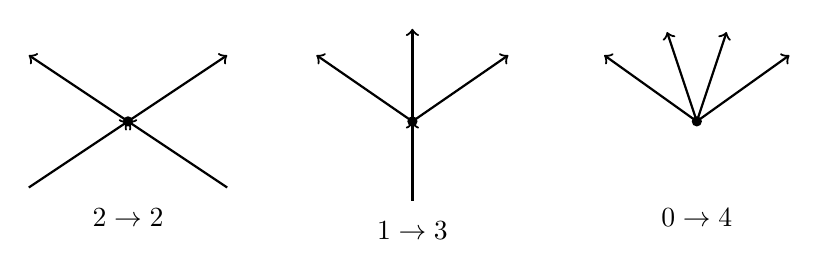
\begin{tikzpicture}[scale=0.84]
\fill (0,0) circle (2.2pt);
\draw[thick,->] (-1.5,-1.0) -- (0,0);
\draw[thick,->] (1.5,-1.0) -- (0,0);
\draw[thick,->] (0,0) -- (-1.5,1.0);
\draw[thick,->] (0,0) -- (1.5,1.0);
\node at (0,-1.45) {$2\to2$};
\begin{scope}[xshift=4.3cm]
\fill (0,0) circle (2.2pt);
\draw[thick,->] (0,-1.2) -- (0,0);
\draw[thick,->] (0,0) -- (-1.45,1.0);
\draw[thick,->] (0,0) -- (0,1.4);
\draw[thick,->] (0,0) -- (1.45,1.0);
\node at (0,-1.65) {$1\to3$};
\end{scope}
\begin{scope}[xshift=8.6cm]
\fill (0,0) circle (2.2pt);
\draw[thick,->] (0,0) -- (-1.4,1.0);
\draw[thick,->] (0,0) -- (-0.45,1.35);
\draw[thick,->] (0,0) -- (0.45,1.35);
\draw[thick,->] (0,0) -- (1.4,1.0);
\node at (0,-1.45) {$0\to4$};
\end{scope}
\end{tikzpicture}
\caption{四腿相互作用頂點的三種局域方向。}
\end{figure}

局域解讀\(0\to4\)本身並不表示四個粒子能在物理過程中從真空中出現。仍須對頂點所有可能的時空位置求和。若假設的外態不符合能量守恆，各位置所帶來的相位便會相消。

\begin{classroomqa}
\lecturetimestamp{01:15:18}
\audiencequestion{四條腿全朝外，是否代表四個粒子自發地出現在末態？}
\lecturerresponse{這是四場算符的一種局域解讀，但沒有入射能量的過程違反能量守恆。把頂點所有可能時空位置的振幅加總後，它們會相消為零。}
\end{classroomqa}

\begin{classroomqa}
\lecturetimestamp{01:15:58}
\audiencequestion{能量守恆與動量守恆是從計算本身得出來的嗎？}
\lecturerresponse{是。對頂點遍及所有時間積分會強制能量守恆；遍及所有空間積分則會強制動量守恆。除非能量和動量都守恆，否則對頂點位置的總和便為零。}
\end{classroomqa}

在這些守恆定律的約束下，拉格朗日量允許的每個圖都會貢獻一定的振幅。貢獻大小部分取決於各相互作用項的係數。將三次與四次係數分別記為\(G_3\)和\(G_4\)。每個三腿頂點帶有一個\(G_3\)因子，每個四腿頂點則帶有一個\(G_4\)因子。因此，含有\(V_3\)個三次頂點與\(V_4\)個四次頂點的圖，其耦合依賴關係示意如下：
\begin{equation}
\mathcal{A}_{\mathrm{graph}}
\propto G_3^{V_3}G_4^{V_4}.
\end{equation}

如果這些耦合很小，頂點較少的圖通常比頂點較多的圖貢獻更大。每多一個頂點，就會多出一個小因子。這讓微擾求和有機會發揮作用：先從最簡單的圖開始，再逐步加入更小的修正。

完整級數是否真的收斂，是個難題。耦合很小時，這種排序看來合理，但光憑小耦合本身仍不能解決所有收斂問題。耦合很大時，樸素級數可能完全失效。這種失效並不表示底層理論有誤；也可能只是表示以耦合常數的冪次展開並不是合適的計算方法。當耦合小到四個頂點的圖遠小於兩個頂點的圖時，這裡討論的方法最能直接派上用場。

\begin{classroomqa}
\lecturetimestamp{01:19:24}
\audiencequestion{色理論也能用同樣的方式處理嗎？}
\lecturerresponse{可以。色理論也能用同樣的方式表述，之後會再討論。}
\end{classroomqa}

\section{傳播子、頂點與互補的描述}

接下來要列出粒子，並以拉格朗日量或費曼規則描述它們的動力學。兩者是同一份資訊的不同形式。二次項描述粒子從一點傳播到另一點；表示這種傳播的線稱為傳播子。涉及三個或更多場的項，則描述線相接之處；這些交會點就是頂點。例如：
\begin{equation}
\begin{aligned}
\text{quadratic term}
&\longleftrightarrow \text{propagator},\\
G_3\phi^3
&\longleftrightarrow \text{three-leg vertex}.
\end{aligned}
\end{equation}

指定一個理論時，可以為每種粒子設一個量子場，並寫出包含所有粒子質量與相互作用的拉格朗日量。等價地，也可以列出每個傳播子、所有允許的頂點，以及各頂點所帶的係數。無論採用哪一種清單，都能指出哪些過程可能發生，以及如何為其圖形指定振幅。

例如，兩個電子可以藉由交換光子而散射。每條電子線上都有一個電子--電子--光子頂點，而光子傳播子則連接這兩個頂點。\footnote{此圖依據01處的例子重構而成：21：38。}

\begin{figure}[htbp]
\centering
\begin{tikzpicture}[scale=0.95]
\draw[->] (-0.6,-0.2) -- (0.2,1.4);
\draw[->] (0.2,1.4) -- (-0.7,3.1);
\draw[->] (3.5,-0.2) -- (2.7,1.4);
\draw[->] (2.7,1.4) -- (3.6,3.1);
\fill (0.2,1.4) circle (2pt);
\fill (2.7,1.4) circle (2pt);
\draw[thick] (0.2,1.4) -- (2.7,1.4);
\node[above] at (1.45,1.4) {$\gamma$};
\node[left] at (-0.2,0.5) {$e^-$};
\node[right] at (3.1,0.5) {$e^-$};
\end{tikzpicture}
\caption{兩個電子透過交換光子而散射。}
\end{figure}

拉格朗日量決定這個圖的振幅，也包含約束振幅的對稱性與守恆定律。在標示時間方向的圖中，底部的粒子構成初態，頂部的粒子構成末態。

\begin{classroomqa}
\lecturetimestamp{01:22:06}
\audiencequestion{費曼圖底部的粒子是初態，頂部的粒子是末態嗎？}
\lecturerresponse{是。底部表示初始粒子組態，頂部表示最終粒子組態。}
\end{classroomqa}

粒子描述與場描述互為補充，就像普通量子力學中動量與位置是互補的描述一樣。它們以不同的基底描述同一個系統，也有相應的不確定性：若粒子數被精確指定，場值就不確定；若場值被精確指定，粒子數就不確定。兩種描述都不能取代另一種，而拉格朗日量在兩者中都適用。

\begin{classroomqa}
\lecturetimestamp{01:23:26}
\audiencequestion{耦合常數是理論預測的，還是由實驗決定的？}
\lecturerresponse{對稱性有時能把不同的耦合常數彼此關聯起來，但它們的數值通常由實驗決定。}
\end{classroomqa}

\section{實驗輸入與廣泛預測}

量子場論本身優雅而美妙。但一旦開始列出各項事實---有哪些粒子、各自的質量，以及耦合常數---這份清單就亂成一團，而且相當難看；除了對稱性帶來的連貫性之外，幾乎毫無章法。對稱性能把不同種類的粒子及其過程關聯起來，但作用有限。大部分粒子資訊仍是一大堆相對零散的事實，描述著一群似乎缺乏明確動機的不同粒子。

\begin{classroomqa}
\lecturetimestamp{01:24:58}
\audiencequestion{為什麼能如此有把握地相信測得的耦合常數？}
\lecturerresponse{耦合常數一旦測定，若改動其數值，預測就會出錯。許多使用該數值的計算都能檢驗它。}
\end{classroomqa}

粒子太多，也就代表場太多---多到難以符合任何審美標準。粒子大約有一百種上下。耦合常數有許多個，數值大多來自實驗；質量也有許多個，分布範圍極廣。它們之間有一些關係，但不多。

但一旦知道這些數值，就可以開始計算。知道之後，便能極精確地計算這些粒子相關的各種性質。夸克、電子、光子等粒子所牽涉的問題，涵蓋原子物理、粒子物理、核子物理、化學，甚至可能還包括生物學。所需的輸入或許比我們希望的多，但能得到的結果非常豐富。

\section{以量子電動力學為微擾例子}

量子電動力學提供了一個耦合常數展開的具體例子。

\begin{classroomqa}
\lecturetimestamp{01:26:12}
\audiencequestion{對電子和光子而言，\(G_n\)型的相互作用耦合有幾個？}
\lecturerresponse{基本相互作用耦合只有一個：電荷\(e\)。它是\(G_3\)型係數，附在一個頂點上；該處有一個電子進入、一個電子離開，並有一個光子發射或吸收。}
\end{classroomqa}

略去旋量矩陣與指標後，相互作用的場內容可示意如下：
\begin{equation}
\mathcal{L}_{\mathrm{QED,int}}
\sim e\,(\text{electron bilinear})\,A,
\end{equation}
其中\(A\)表示光子場。計數時不需要用到狄拉克矩陣的詳細結構。量子電動力學的基本規則是電子發射或吸收光子；所有更複雜的量子電動力學圖，都由反覆使用這個頂點組成。\footnote{此示意頂點依據01處的內容重構：26：42；原文刻意略去矩陣的詳細結構。}

\begin{figure}[htbp]
\centering
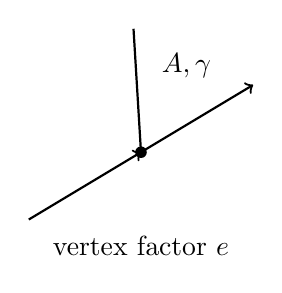
\begin{tikzpicture}[scale=0.95]
\draw[thick,->] (-1.5,-0.9) -- (0,0);
\draw[thick,->] (0,0) -- (1.5,0.9);
\draw[thick] (0,0) -- (-0.1,1.65);
\fill (0,0) circle (2.2pt);
\node[right] at (0.15,1.15) {$A,\gamma$};
\node at (0,-1.25) {vertex factor $e$};
\end{tikzpicture}
\caption{量子電動力學中基本的電子--電子--光子頂點。}
\end{figure}

\begin{classroomqa}
\lecturetimestamp{01:27:38}
\audiencequestion{電子--質子散射又是怎麼回事？}
\lecturerresponse{在基礎的原子物理處理中，可以把質子理想化為固定且無限重的點源---也就是一個被釘在原處的重粒子。只有在納入質子與中子的內部理論時，才需要考慮它們自身的量子場動力學。}
\end{classroomqa}

\begin{classroomqa}
\lecturetimestamp{01:28:30}
\audiencequestion{電子相對於那個質子，能以接近光速的速度運動嗎？}
\lecturerresponse{可以。}
\end{classroomqa}

考慮光子被電子散射。在最低階，圖中有兩個電子--電子--光子頂點，因此振幅正比於\(e^2\)：
\begin{equation}
\mathcal{A}_{\mathrm{lowest}}\propto e^2.
\end{equation}
散射機率，或等價地說，截面對耦合常數的依賴關係，來自振幅的絕對值平方，正比於\(e^4\)：
\begin{equation}
P_{\mathrm{lowest}}\ \text{or}\ \sigma_{\mathrm{lowest}}
\propto e^4.
\end{equation}
採用慣用的無因次歸一化時，電耦合很小，因此光子真正發生散射的機率，遠低於它直接通過而不散射的機率。

在這一階已經有兩個圖。一種時間順序是先吸收入射光子，稍後再發射出射光子；另一種則是先發射出射光子，之後才吸收入射光子。兩種振幅都會有所貢獻。\footnote{這兩種時間順序依據01：28：42與01：30：18處的圖示重構而成。}

\begin{figure}[htbp]
\centering
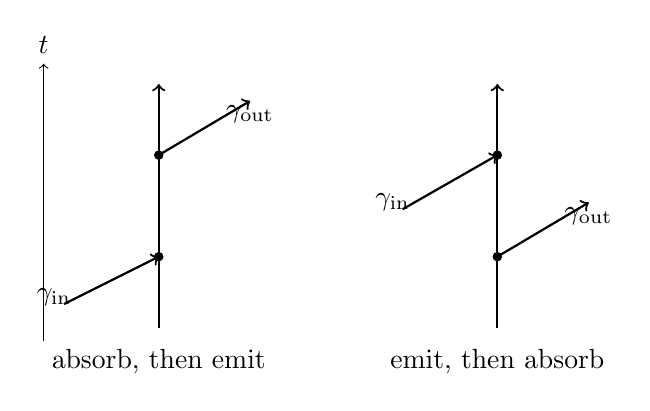
\begin{tikzpicture}[scale=0.86]
\draw[->] (-0.7,0) -- (-0.7,4.1) node[above] {$t$};
\draw[thick,->] (1.0,0.2) -- (1.0,3.8);
\fill (1.0,1.25) circle (2pt);
\fill (1.0,2.75) circle (2pt);
\draw[thick,->] (-0.4,0.55) -- (1.0,1.25);
\draw[thick,->] (1.0,2.75) -- (2.35,3.55);
\node[left] at (-0.15,0.65) {$\gamma_{\mathrm{in}}$};
\node[right] at (1.85,3.35) {$\gamma_{\mathrm{out}}$};
\node at (1.0,-0.3) {absorb, then emit};
\begin{scope}[xshift=5.0cm]
\draw[thick,->] (1.0,0.2) -- (1.0,3.8);
\fill (1.0,1.25) circle (2pt);
\fill (1.0,2.75) circle (2pt);
\draw[thick,->] (1.0,1.25) -- (2.35,2.05);
\draw[thick,->] (-0.4,1.95) -- (1.0,2.75);
\node[right] at (1.85,1.85) {$\gamma_{\mathrm{out}}$};
\node[left] at (-0.15,2.05) {$\gamma_{\mathrm{in}}$};
\node at (1.0,-0.3) {emit, then absorb};
\end{scope}
\end{tikzpicture}
\caption{電子--光子散射的兩種最低階時間順序。}
\end{figure}

因此，最低階振幅不是單一圖形，而是兩個振幅的總和：
\begin{equation}
\begin{aligned}
\mathcal{A}^{(2)}
&=
\mathcal{A}_{\mathrm{absorb\ then\ emit}}
+\mathcal{A}_{\mathrm{emit\ then\ absorb}},\\
\mathcal{A}^{(2)}&\propto e^2.
\end{aligned}
\end{equation}

高階修正會加入更多基本頂點。額外的內部光子若在電子線上連接兩次，就會多出兩個\(e\)因子，使振幅中的貢獻正比於\(e^4\)，其絕對值平方則正比於\(e^8\)。光子線中也可能插入電子--正電子對，這同樣會加入基本頂點及更多\(e\)次方。這些只是例子，並非完整列舉；額外光子可以接在許多不同位置。\footnote{高階結構依據01：30：38--01：31：16處的圖示重構而成。}

\begin{figure}[htbp]
\centering
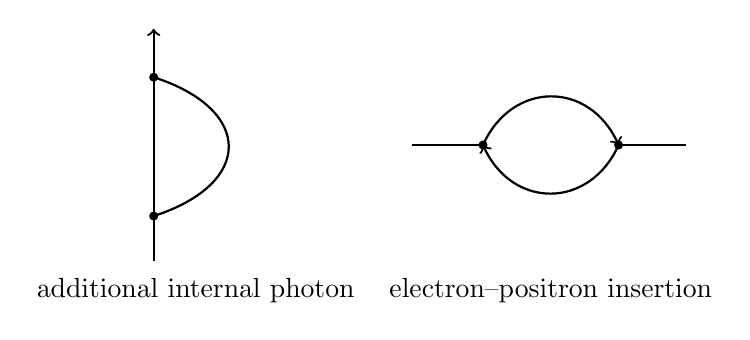
\begin{tikzpicture}[scale=0.82]
\draw[thick,->] (0.9,0.2) -- (0.9,3.8);
\fill (0.9,0.9) circle (2pt);
\fill (0.9,3.05) circle (2pt);
\draw[thick] (0.9,0.9) .. controls (2.45,1.4) and (2.45,2.55) .. (0.9,3.05);
\node at (1.55,-0.25) {additional internal photon};
\begin{scope}[xshift=5.1cm]
\draw[thick] (-0.2,2.0) -- (0.9,2.0);
\fill (0.9,2.0) circle (2pt);
\fill (3.0,2.0) circle (2pt);
\draw[thick,->] (0.9,2.0) .. controls (1.35,3.0) and (2.55,3.0) .. (3.0,2.0);
\draw[thick,->] (3.0,2.0) .. controls (2.55,1.0) and (1.35,1.0) .. (0.9,2.0);
\draw[thick] (3.0,2.0) -- (4.05,2.0);
\node at (1.95,-0.25) {electron--positron insertion};
\end{scope}
\end{tikzpicture}
\caption{兩種加入基本頂點、因而帶有更多\(e\)次方的高階 QED 結構。}
\end{figure}

因此，QED 展開依照\(e^2\)的次方逐階進行。每增加一項程度相當的新複雜結構，振幅中就會多出電荷的兩次方。在所採用的歸一化下，這類修正在振幅上大約比前一階小一百倍或兩百倍。越複雜的圖，貢獻就越小，因此微擾求和有機會發揮作用。

機率不是先分別將每個圖的振幅平方，再把平方結果相加。應先將對同一外部過程有貢獻的所有振幅加總：
\begin{equation}
\mathcal{A}_{\mathrm{total}}=\sum_r\mathcal{A}_r.
\end{equation}
然後才計算
\begin{equation}
P=\left|\mathcal{A}_{\mathrm{total}}\right|^2
=\left|\sum_r\mathcal{A}_r\right|^2.
\end{equation}
不同圖之間的交叉項就是干涉項。規則簡單而且關鍵：先相加，再取平方。

\section{邁向粒子清單與標準模型}

有了傳播子、頂點、耦合常數計數與干涉，粒子物理的描述便能正式展開。我們可以為粒子命名、指定它們的質量，寫出部分由理論、部分由實驗決定的支配其行為的拉格朗日量，並直接研究其中的對稱性。同一套架構接著會導向標準模型及其性質。

\begin{classroomqa}
\lecturetimestamp{01:33:22}
\audiencequestion{可以用希格斯場取代固定的質量係數\(m^2\)嗎？}
\lecturerresponse{可以。這個想法是對的，之後會討論這種機制。}
\end{classroomqa}

\begin{classroomqa}
\lecturetimestamp{01:33:42}
\audiencequestion{相鄰的點陣點\(x\)和\(x'\)可以位於不同的時間嗎？}
\lecturerresponse{可以。它們可以沿時間方向相鄰；點陣上的縱向傳播就是這樣表示的。}
\end{classroomqa}

對相鄰點而言，有限差分的平方同時包含同點項與跨連線項：
\begin{equation}
\bigl[\phi(x)-\phi(x')\bigr]^2
=
\phi(x)^2+\phi(x')^2-2\phi(x)\phi(x').
\end{equation}

\begin{classroomqa}
\lecturetimestamp{01:33:56}
\audiencequestion{哪一項代表粒子只是停在原處？}
\lecturerresponse{有限差分平方中的同點項\(\phi(x)^2\)與\(\phi(x')^2\)代表粒子停在原處，而交叉項\(\phi(x)\phi(x')\)則對應粒子移動。顯式的質量項也會貢獻同點、靜止不動的因子。}
\end{classroomqa}
